% 原书印刷144–151／物理169–176，止于实际§4.4标题前.
\subsection{运输密度的可积性}\label{sec:4.3}\index{T151@传输密度（transport density）|hyperpage}
\setcounter{theorem}{15}\setcounter{equation}{10}\setcounter{figure}{1}\setcounter{footnote}{3}
前几节对Beckmann问题的分析主要在测度框架中进行，最优$\mathbf w$与运输密度$\sigma$只是$\Omega$上的测度. 这里研究的问题是：对$\mu$和／或$\nu$施加额外假设后，它们是否具有额外正则性.

我们将给出可积性结果，证明$\sigma$在某些情形下绝对连续，并给出$L^p$估计. 证明主要取自\cite{b273}，另见\cite{b61,b166}；更早的结果最初由\cite{b143,b144,b145}通过很不相同的技术给出. 这些论文还给出$\sigma$的“维数”的不同估计，因此在$\sigma$不绝对连续时，也能提供有趣信息. \phantomsection\label{idx:root4-p144-image-processing}\index{I077@图像处理（image processing）|hyperpage}还应指出，\cite{b208}在将这些工具应用于图像处理时，给出了一个新的\footnote{他们的证明介于\cite{b143}的证明与本书这里的证明之间：与这里一样，\cite{b208}也采用原子测度逼近，但同时逼近源测度和目标测度，因此需要像\cite{b143}那样对运输射线进行几何分析.}绝对连续性证明.

注意，更高阶的问题，例如当$\mu$与$\nu$具有光滑密度时，$\sigma$是否连续、Lipschitz连续或更正则，迄今仍完全未解. 唯一例外是二维中的一个部分结果，见\cite{b171}：当$\mu$和$\nu$在互不相交的凸区域上具有Lipschitz密度时，可以得到连续性.

\begin{openproblem}[运输密度的连续性]
假设$\mu,\nu$有连续密度，运输密度$\sigma$是否也连续？若它们Lipschitz连续，$\sigma$是否也Lipschitz连续；以及／或者，若它们Hölder连续，$\sigma$是否也Hölder连续？
\end{openproblem}
下文始终假设$\Omega$是$\mathbb R^d$中的紧凸区域，并在其上给定两个概率测度$\mu,\nu$. 其中至少一个绝对连续，从而$\sigma$唯一，见\autoref{obj:4.14}. 第一个结果最初在\cite{b162}中得到，涉及$L^1$可积性，即绝对连续性.

\begin{theorem}\label{obj:4.16}
假设$\Omega\subset\mathbb R^d$为凸区域，且$\mu\ll\mathscr L^d$. 令$\sigma$为与从$\mu$到$\nu$的运输关联的运输密度. 则$\sigma\ll\mathscr L^d$.
\end{theorem}
\begin{proof}
取从$\mu$到$\nu$的一个最优运输方案$\gamma$，并令$\sigma=\sigma_\gamma$；以$\mu_t$表示两测度之间的标准插值：$\mu_t=(\pi_t)_\#\gamma$，其中$\pi_t(x,y)=(1-t)x+ty$. 有$\mu_0=\mu$、$\mu_1=\nu$.

我们已经看到，回顾\eqref{eq:4.6}，运输密度$\sigma$可写成
\[
\sigma=\int_0^1(\pi_t)_\#(c\cdot\gamma)\,dt,
\]
其中$c:\Omega\times\Omega\to\mathbb R$是成本函数$c(x,y)=|x-y|$，从而$c\cdot\gamma$为$\Omega\times\Omega$上的正测度.

由于$\Omega$有界，显然有
\begin{equation}\label{eq:4.11}
\sigma\leq C\int_0^1\mu_t\,dt.
\end{equation}
要证明$\sigma$绝对连续，只须证明几乎每个测度$\mu_t$都绝对连续：如此一来，只要$|A|=0$，便有$\sigma(A)\leq C\int_0^1\mu_t(A)\,dt=0$.

我们将证明$t<1$时$\mu_t\ll\mathscr L^d$. 首先假设$\nu$是有限原子测度，以$(x_i)_{i=1,\ldots,N}$为其原子. 此时，选择任意一个由运输映射$\mathrm T$诱导的最优运输方案$\gamma$；由于$\mu\ll\mathscr L^d$，这样的映射存在. 注意，$\sigma$的绝对连续性很容易由从$\mu$到$\nu$的最优运输的行为得到，因为该运输由$N$个位似组成；但我们还希望定量刻画这种绝对连续性，以便进行逼近.

回顾$\mu$绝对连续，因此存在对应关系$\varepsilon\mapsto\delta=\delta(\varepsilon)$，满足
\begin{equation}\label{eq:4.12}
|A|<\delta(\varepsilon)\quad\Longrightarrow\quad\mu(A)<\varepsilon.
\end{equation}
现在取一个Borel集$A$，考察$\mu_t(A)$. 区域$\Omega$是不交的有限个集合$\Omega_i=\mathrm T^{-1}(\{x_i\})$之并. 以$\Omega_i(t)$表示$\Omega_i$通过映射$x\mapsto(1-t)x+t\mathrm T(x)$得到的像，见\autoref{fig:4.2}. 这些集合本质上不相交. 为什么？若某点$z$同时属于$\Omega_i(t)$和$\Omega_j(t)$，则两条运输射线在$z$相交：一条从$x_i'\in\Omega_i$到$x_i$，另一条从$x_j'\in\Omega_j$到$x_j$. 唯一的可能是这两条射线实际上相同，即$x_i',x_j',z,x_i,x_j$这五点共线. 但这说明$z$属于连接两个原子$x_i,x_j$的某条直线. 由于这样的直线只有有限条，其并集是零测集. 注意，这一论证只适用于$d>1$；我们不在$d=1$的情形上多花时间，因为这时运输密度总是BV函数，因而有界. 而且，若始终选择沿射线单调的最优运输映射，实际上可以证明这些集合真正不相交，而非仅交于零测集.

于是有
\begin{equation*}\begin{aligned}
\mu_t(A)&=\sum_i\mu_t(A\cap\Omega_i(t))\\
&=\sum_i\mu_0\left(\frac{A\cap\Omega_i(t)-tx_i}{1-t}\right)
=\mu_0\left(\bigcup_i\frac{A\cap\Omega_i(t)-tx_i}{1-t}\right).
\end{aligned}\end{equation*}
由于对每个$i$都有
\[
\left|\frac{A\cap\Omega_i(t)-tx_i}{1-t}\right|
=\frac{1}{(1-t)^d}|A\cap\Omega_i(t)|,
\]
可得
\[
\left|\bigcup_i\frac{A\cap\Omega_i(t)-tx_i}{1-t}\right|
\leq\frac{1}{(1-t)^d}|A|.
\]
因而，只需假设$|A|<(1-t)^d\delta(\varepsilon)$，就得到$\mu_t(A)<\varepsilon$. 这确认了$\mu_t\ll\mathscr L^d$，并给出一个可以传递到极限的估计.

\begin{figure}[htbp]\centering
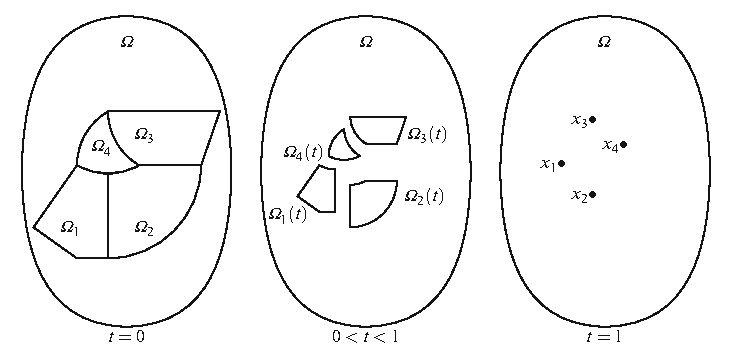
\includegraphics[width=.95\textwidth]{assets/ch04b-fig4-2.pdf}
\caption{集合$\Omega_i(t)$的不交性.}\label{fig:4.2}
\end{figure}

取一列收敛到$\nu$的原子测度$\nu^n$. 相应的最优运输方案$\gamma^n$收敛到某个最优运输方案$\gamma$，而$\mu_t^n$收敛到相应的$\mu_t$，见\autoref{sec:1}的\autoref{obj:1.50}. 因此，要证明与此$\gamma$关联的运输密度$\sigma$绝对连续，只须证明这些$\mu_t$绝对连续.

取满足$|A|<(1-t)^d\delta(\varepsilon)$的集合$A$. 由于Lebesgue测度正则，见\autoref{box:1.6}中的定义，$A$包含于某个开集$B$，且$|B|<(1-t)^d\delta(\varepsilon)$. 因而$\mu_t^n(B)<\varepsilon$. 根据弱收敛以及在开集上的半连续性，取极限得到
\[
\mu_t(A)\leq\mu_t(B)\leq\liminf_n\mu_t^n(B)\leq\varepsilon.
\]
这证明了$\mu_t\ll\mathscr L^d$，从而$\sigma\ll\mathscr L^d$.
\end{proof}

\begin{remark}\label{obj:4.17}
我们在哪里使用了$\gamma$的最优性？在断言$\Omega_i(t)$互不相交时. 对于离散测度$\nu$，与任意运输方案$\gamma$对应的测度$\mu_t$，在$t<1$时总是绝对连续的；但是，若允许$\Omega_i(t)$相互重叠，其绝对连续性就可能在极限中退化，因为这时密度会相加，估计可能依赖于原子数.
\end{remark}
\begin{remark}\label{obj:4.18}
注意，我们强烈依赖于绝对连续性两种定义的等价：一方面是$\varepsilon\leftrightarrow\delta$对应，另一方面是关于零测集的条件. 要证明条件$\mu_t\ll\mathscr L^d$可以传递到极限，需要前者；要推出$\sigma\ll\mathscr L^d$，则需要后者.
\end{remark}

\begin{figure}[htbp]\centering
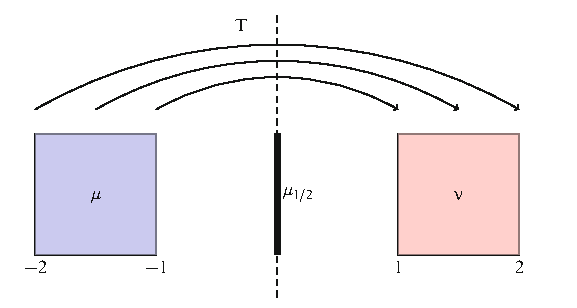
\includegraphics[width=.78\textwidth]{assets/ch04b-fig4-3.pdf}
\caption{一个不能由第二边缘为原子测度的最优方案逼近的最优运输方案的例子.}\label{fig:4.3}
\end{figure}
\begin{remark}\label{obj:4.19}
作为证明的副产品，可以看出：从$\mu$到$\nu$的任何最优运输方案，只要能够通过从$\mu$到原子测度的最优运输方案逼近，就必然满足所有插值测度$\mu_t$在每个$t\in]0,1[$时都绝对连续. 并非每个最优运输方案都有此性质. 例如，将$\mu=\mathscr L^2\restr([-2,-1]\times[0,1])$通过$(x,y)\mapsto(-x,y)$送到$\nu=\mathscr L^2\restr([1,2]\times[0,1])$的方案$\gamma$是最优的，但有$\mu_{1/2}=\mathscr H^1\restr(\{0\}\times[0,1])$. 因而，此方案不能被把$\mu$送往原子测度的最优方案逼近. 另一方面，我们在\autoref{obj:3.20}中证明，单调最优运输确实可以用类似方式逼近，见\autoref{fig:4.3}.
\end{remark}
从现在起，我们经常将绝对连续测度与其密度混用：当$\mu=f\cdot\mathscr L^d$时，将$\|f\|_{L^p(\Omega)}$记为$\|\mu\|_{L^p}$.

\begin{theorem}\label{obj:4.20}
假设$\mu=f\cdot\mathscr L^d$，其中$f\in L^p(\Omega)$，$\Omega$紧且凸. 若$p<d':=d/(d-1)$，则从$\mu$到$\nu$的运输所关联的唯一运输密度$\sigma$也属于$L^p(\Omega)$；若$p\geq d'$，则它属于每个$q<d'$对应的$L^q(\Omega)$.
\end{theorem}
\begin{proof}
先考虑$p<d'$：沿用前面的策略与记号，只须证明每个$t\in[0,1[$对应的测度$\mu_t$都属于$L^p$，并估计其$L^p$范数. 然后使用
\[
\|\sigma\|_{L^p}\leq C\int_0^1\|\mu_t\|_{L^p}\,dt,
\]
它由\eqref{eq:4.11}与Minkowski不等式得到；对$p$施加的条件，恰好为了使此积分收敛.

先考虑离散情形：已知$\mu_t$绝对连续，其密度在每个集合$\Omega_i(t)$上，等于$\mu$在$\Omega_i$上以比例$1-t$作位似后的密度. 因此，若$f_t$为$\mu_t$的密度，则
\begin{equation*}\begin{aligned}
\int_\Omega f_t(x)^p\,dx
&=\sum_i\int_{\Omega_i(t)}f_t(x)^p\,dx\\
&=\sum_i\int_{\Omega_i}\left(\frac{f(x)}{(1-t)^d}\right)^p(1-t)^d\,dx\\
&=(1-t)^{d(1-p)}\sum_i\int_{\Omega_i}f(x)^p\,dx
=(1-t)^{d(1-p)}\int_\Omega f(x)^p\,dx.
\end{aligned}\end{equation*}
得到$\|\mu_t\|_{L^p}=(1-t)^{-d/p'}\|\mu\|_{L^p}$，其中$p'=p/(p-1)$.

这一不等式在离散情形成立，在极限中也仍然成立. 若$\nu$不是原子测度，通过一列$\mu_1^n$来逼近它，并取最优方案$\gamma^n$及插值测度$\mu_t^n$. 抽取子列后，有$\gamma^n\rightharpoonup\gamma$，其中$\gamma$是最优运输方案；并有$\mu_t^n\rightharpoonup\mu_t$，后者为相应插值. 由半连续性，
\[
\|\mu_t\|_{L^p}\leq\liminf_n\|\mu_t^n\|_{L^p}
\leq(1-t)^{-d/p'}\|\mu_0\|_{L^p},
\]
于是
\[
\|\sigma\|_{L^p}\leq C\int_0^1\|\mu_t\|_{L^p}\,dt
\leq C\|\mu_0\|_{L^p}\int_0^1(1-t)^{-d/p'}\,dt.
\]
最后一个积分有限，只要$p'>d$，即$p<d'=d/(d-1)$.

陈述的第二部分，即$p\geq d'$的情形，直接由$L^p$中的密度也属于每个$q<p$对应的$L^q$空间得到.
\end{proof}

\begin{example}\label{obj:4.21}
下面的例子说明，即使$\mu\in L^\infty$，$\nu$的奇性也可能使$\sigma$不属于$L^{d'}$. 取$\mu=f\cdot\mathscr L^d$，其中$f=\mathbf1_A$、$A=B(0,R)\setminus B(0,R/2)$，并选择$R$使$\int f=1$；取$\nu=\delta_0$. 注意$\frac R2\gamma\leq c\cdot\gamma\leq R\gamma$，这说明
\[
\sigma=\int_0^1(\pi_t)_\#(c\cdot\gamma)\,dt
\]
的可积性，与$\int_0^1(\pi_t)_\#\gamma\,dt=\int_0^1\mu_t\,dt$相同. 有$\mu_t=f_t\cdot\mathscr L^d$，其中$f_t=(1-t)^{-d}\mathbf1_{(1-t)A}$；因而
\[
\int_0^1f_t(x)\,dt=\int_{|x|/R}^{2|x|/R}\frac1{s^d}\,ds
=c|x|^{1-d}\qquad\text{当 }|x|\leq\frac R2,
\]
这里使用换元$s=1-t$. 在$d$维空间中，该函数在原点邻域属于$L^p$，当且仅当$(1-d)p+(d-1)>-1$，即$(d-1)(p-1)<1$. 这恰好就是$p<d'$.
\end{example}

在前面几个定理中，我们看到，测度$\mu_t$从$\mu$继承某种正则性，即绝对连续性或$L^p$可积性，其行为与比例为$1-t$的位似完全相同. 这种正则性在$t\to1$时退化，但我们已看到两种不受该退化影响的情形：证明绝对连续性时，几乎所有$\mu_t$各自绝对连续就已足够；对于$L^p$估计，只要该退化仍然可积，也没有问题.

自然可以尝试另一策略：假设$\mu$和$\nu$都满足某种正则性条件，例如都属于$L^p$. 那么，$t\leq1/2$时从$\mu$出发估计$\mu_t$，$t\geq1/2$时从$\nu$出发估计. 如此便没有退化！

这一策略相当有效，但还有额外困难：在先前估计中，并非事先知道$\mu_t$与$\mu$的分片位似具有相同行为，而是将其作为离散逼近的极限得到. 取极限时，不知道最优方案$\gamma^n$会选择哪个最优运输$\gamma$作为极限. 在前一节中这并不重要，因为任意最优$\gamma$都诱导同一个运输密度$\sigma$. 但这里，希望把逼近$\mu_1$所得的$t\leq1/2$的估计，与逼近$\mu_0$所得的$t\geq1/2$的估计拼接起来. 若这两种逼近收敛到不同运输方案，就不能合并两组估计，也无法推出关于$\sigma$的结论.

因此，需要考虑的主要技术问题是证明某个特定最优运输方案，即沿射线单调的方案，能够从两个方向逼近. \autoref{obj:3.20}恰好完成这一任务；事实上，\cite{b273}证明它正是为此. 不过，逼近时构造的运输方案$\gamma_\varepsilon$并非对成本$|x-y|$最优，而是对某些成本$|x-y|+\varepsilon|x-y|^2$最优. 这样做是为了通过一个次级变分问题，强制所选极限最优运输为单调方案. 无论如何，这并不构成问题：这些逼近的最优运输方案具有相同几何性质，能够保证$\Omega_i(t)$互不相交. 特别地，可以证明如下估计.

\begin{lemma}\label{obj:4.22}
设$\gamma$为$\mu$与原子测度$\nu$之间、关于成本$c(x,y)=h(y-x)$的最优运输方案，其中$h:\mathbb R^d\to\mathbb R$严格凸. 照例令$\mu_t=(\pi_t)_\#\gamma$. 则
\[
\|\mu_t\|_{L^p}\leq(1-t)^{-d/p'}\|\mu\|_{L^p}.
\]
\end{lemma}
\begin{proof}
结果与\autoref{obj:4.20}完全相同，关键工具是$\mu_t$在每个$\Omega_i(t)$上与$\mu_0$的一个位似像相同. 唯一需要重新核查的是$\Omega_i(t)$的不交性.

为此，取$x\in\Omega_i(t)\cap\Omega_j(t)$. 则存在分别属于$\Omega_i$和$\Omega_j$的$x_i,x_j$，使$x=(1-t)x_i+ty_i=(1-t)x_j+ty_j$，其中$y_i=\mathrm T(x_i)$与$y_j=\mathrm T(x_j)$是$\nu$的两个原子. 这说明$\mathrm T_t:=(1-t)\operatorname{id}+t\mathrm T$不是单射，与下面的\autoref{obj:4.23}矛盾. 因而$\Omega_i(t)$互不相交，从而得到$\mu_t$的界.
\end{proof}

\begin{lemma}\label{obj:4.23}
设$\gamma$为$\mu$与$\nu$之间、关于成本$c(x,y)=h(y-x)$的最优运输方案，其中$h:\mathbb R^d\to\mathbb R$严格凸，并假设它由运输映射$\mathrm T$诱导. 选择$\mathrm T$的一个代表元，使每个$x$都满足$(x,\mathrm T(x))\in\operatorname{spt}(\gamma)$. 则映射$x\mapsto(1-t)x+t\mathrm T(x)$在$t\in]0,1[$时为单射.
\end{lemma}
\begin{proof}
假设存在$x\ne x'$，使
\[
(1-t)x+t\mathrm T(x)=(1-t)x'+t\mathrm T(x')=x_0.
\]
令$a=\mathrm T(x)-x$、$b=\mathrm T(x')-x'$. 这也意味着$x=x_0-ta$、$x'=x_0-tb$. 特别地，由$x\ne x'$得到$a\ne b$.

最优$\gamma$的支集的$c$-循环单调性给出
\begin{equation*}\begin{aligned}
h(a)+h(b)&\leq h(\mathrm T(x')-x)+h(\mathrm T(x)-x')\\
&=h(tb+(1-t)a)+h(ta+(1-t)b).
\end{aligned}\end{equation*}
然而$a\ne b$，严格凸性意味着
\begin{equation*}\begin{aligned}
&h(tb+(1-t)a)+h(ta+(1-t)b)\\
&\quad<th(b)+(1-t)h(a)+th(a)+(1-t)h(b)
=h(a)+h(b),
\end{aligned}\end{equation*}
矛盾.
\end{proof}

\begin{theorem}\label{obj:4.24}
假设$\mu$、$\nu$是$\Omega$上的概率测度，且都属于$L^p(\Omega)$；令$\sigma$为从$\mu$到$\nu$的运输所关联的唯一运输密度. 则$\sigma$也属于$L^p(\Omega)$.
\end{theorem}
\begin{proof}
考虑由\eqref{eq:3.4}定义的从$\mu$到$\nu$的最优运输方案$\bar\gamma$. 已知此方案可以由方案$\gamma^\varepsilon$逼近，后者对于成本$|x-y|+\varepsilon|x-y|^2$，在从$\mu$到某些离散原子测度$\nu_\varepsilon$的运输中最优. 相应插值测度$\mu_t^\varepsilon$满足\autoref{obj:4.22}的$L^p$估计；在极限中，
\[
\|\mu_t\|_{L^p}\leq\liminf_{\varepsilon\to0}\|\mu_t^\varepsilon\|_{L^p}
\leq(1-t)^{-d/p'}\|\mu\|_{L^p}.
\]
同样的估计可以从另一方向进行，因为同一个运输方案$\bar\gamma$也可以被关于成本$|x-y|+\varepsilon|x-y|^2$、从原子测度到$\nu$的最优方案逼近. 合并两组估计，得到
\begin{equation*}\begin{aligned}
\|\mu_t\|_{L^p}
&\leq\min\left\{(1-t)^{-d/p'}\|\mu\|_{L^p},t^{-d/p'}\|\nu\|_{L^p}\right\}\\
&\leq2^{d/p'}\max\{\|\mu\|_{L^p},\|\nu\|_{L^p}\}.
\end{aligned}\end{equation*}
对这些$L^p$范数积分，便得到$\|\sigma\|_{L^p}$的界.
\end{proof}

\begin{remark}\label{obj:4.25}
借助泛函$\mu\mapsto\|\mu\|_{L^p}^p$的位移凸性，可以用一种很不相同的方式得到同一结果. 实际上，对$q>1$，此泛函沿空间$\mathbb W_q(\Omega)$中的测地线凸，见\autoref{obj:7.29}；可惜那里$p$与$q$的记号正好相反. 随后令$q\to1$：这就给出与$K_q$-最优方案的极限对应的最优方案之插值测度的结果. 顺便说，这个方案仍然是$\bar\gamma$. 积分估计也随之直接得到. 不过，这需要比目前已发展的工具更精细的工具.
\end{remark}

\begin{example}\label{obj:4.26}
在高于一维的情形，可以举出$\sigma$的可积性不优于$\mu,\nu$的例子. 例如，取$\mu=f\cdot\mathscr L^d$、$\nu=g\cdot\mathscr L^d$，其中
\begin{align*}
f(x_1,x_2,\ldots,x_d)&=f_0(x_2,\ldots,x_d)\mathbf1_{[0,1]}(x_1),\\
g(x_1,x_2,\ldots,x_d)&=f_0(x_2,\ldots,x_d)\mathbf1_{[4,5]}(x_1).
\end{align*}
不难验证，此例的运输射线沿第一坐标向量方向，最优$\sigma$绝对连续，其密度为$\sigma(x)=f_0(x_2,\ldots,x_d)s(x_1)$，其中$s:\mathbb R\to\mathbb R_+$由$s'=\mathbf1_{[0,1]}-\mathbf1_{[4,5]}$、$s(0)=s(5)=0$刻画；这来自$s$是$\mathbf1_{[0,1]}$与$\mathbf1_{[4,5]}$之间一维运输的运输密度. 因而，由$s=1$在$[1,4]$上成立，可见$\sigma$的可积性与$f_0$相同，也就与$f,g$相同.
\end{example}
